\ifnotes
\else
  \PassOptionsToClass{handout}{beamer}
\fi

\documentclass[10pt,t]{beamer}

\usetheme{metropolis} % use metropolis theme

\usepackage{solarized}            % use solarized themed listings
\usepackage{appendixnumberbeamer} % do not number appendix frames
\usepackage[scale=3]{ccicons}     % creative commons icons

% fix-up the handling of the notes pages
\ifnotes
  \hypersetup{final}
  \usepackage{pgfpages}
  \setbeamertemplate{note page}[plain]
  \setbeameroption{show notes on second screen=right}
\fi

%-------------------------------------------------------------------------------

\usepackage{tabularx}
\usepackage{tikz}
\usetikzlibrary{decorations.pathreplacing}

\title{Introduction to MPI}
\date{}
\author{Jeremy Iverson}
\institute{College of Saint Benedict \& Saint John's University}
\begin{document}
  \maketitle

  \begin{frame}{background}
    \begin{center}
      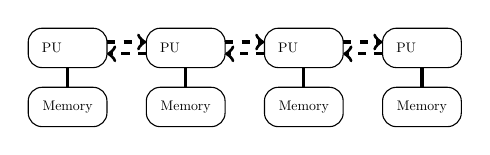
\begin{tikzpicture}[scale=.5,every node/.style={transform shape}]
        \foreach \x in {0,3,6,9}
        {
          \draw[rounded corners=5pt] (\x,-7) rectangle ++(2,1);
          \node at ({\x+.6},-6.5) {PU};

          \draw[very thick] ({\x+1},-7.5) -- ({\x+1},-7);
          \draw[rounded corners=5pt] (\x,-8.5) rectangle ++(2,1);
          \node at ({\x+1},-8) {Memory};
        }
        \foreach \u/\v in {2/3,5/6,8/9}
        {
          \draw[very thick,dashed,->] (\u,-6.35) -- (\v,-6.35);
          \draw[very thick,dashed,->] (\v,-6.65) -- (\u,-6.65);
        }
      \end{tikzpicture}
    \end{center}

    \begin{itemize}
      \item A standard for explicit distributed memory parallel computation.
      \item Many implementations available, both open-source and proprietary.
    \end{itemize}

    \note[item] { We are using an implementation of MPI called Open-MPI }
  \end{frame}


  \begin{frame}{execution model}
    \begin{itemize}
      \item Uses the \emph{SPMD} model of parallelism
        \begin{itemize}
          \item All processes execute the same program.
            \begin{itemize}
              \item Different processes carry out different actions by
                conditional execution of code based on processes' rank.
              \item Processes can communicate with each other by sending
                explicit messages
            \end{itemize}
        \end{itemize}
    \end{itemize}
  \end{frame}

  \begin{frame}{library api}
    \begin{itemize}
      \item Requires inclusion of \texttt{mpi.h} header file.
    \end{itemize}

    \begin{itemize}
      \item \texttt{MPI\_Init()}
      \item \texttt{MPI\_Finalize()}
      \item \texttt{MPI\_Comm\_size()}
      \item \texttt{MPI\_Comm\_rank()}
      \item \texttt{MPI\_Send()}
      \item \texttt{MPI\_Recv()}
    \end{itemize}

    \begin{itemize}
      \item MPI uses \emph{communicators} to organize processes. Processes can
        only communicate with other processes in the same communicator. The base
        communicator to which all processes belong is called
        \texttt{MPI\_COMM\_WORLD}.

      \item Programs can deadlock due to improperly ordered or unmatched
        point-to-point communications.
    \end{itemize}
  \end{frame}

  \appendix

  \begin{frame}[c]
    \begin{center}\ccbysa\end{center}

    except where otherwise noted, this worked is licensed under
    \href{http://creativecommons.org/licenses/by-sa/4.0/}{creative commons
    attribution-sharealike 4.0 international license}
  \end{frame}
\end{document}
